\documentclass[a4paper,10pt,oneside,final,titlepage,onecolumn]{article}

\usepackage{ucs}
\usepackage[portuguese]{babel}
\usepackage[utf8x]{inputenc}
\usepackage[T1]{fontenc}
\usepackage{textcomp}
\usepackage{graphicx}
\usepackage{placeins}

\usepackage{listings}
\usepackage{color}

\definecolor{dkgreen}{rgb}{0,0.6,0}
\definecolor{gray}{rgb}{0.5,0.5,0.5}
\definecolor{mauve}{rgb}{0.58,0,0.82}

\lstset{frame=tb,
  language=bash,
  aboveskip=3mm,
  belowskip=3mm,
  showstringspaces=false,
  columns=flexible,
  basicstyle={\scriptsize\ttfamily},
  numbers=none,  
  breaklines=true,
  breakatwhitespace=true
  tabsize=3
}



\title{Exercício 3 de MC833 --- Programação em Redes de Computadores}
\author{Raul Rabelo Carvalho, 105607, turma A}



\begin{document}



\maketitle



\section{}
\paragraph{}A figura \ref{print-ipport-client} mostra o cliente imprimindo na saída padrão o endereço IP e a porta associados à conexão pelo sistema operacional. O servidor está sendo executado no \emph{host} \verb|guns.lab.ic.unicamp.br:10101| (\verb|143.106.16.5:10101) e o cliente, no \emph{host} em \verb|143.106.16.163|. O endereço IP e a porta impressas pelo cliente são confirmadas pela linha destacada na saída do comando \verb|netstat -tun|.
\begin{figure}[!ht]
  \caption{Cliente imprimindo o endereço IP e a porta.}
  \centering
  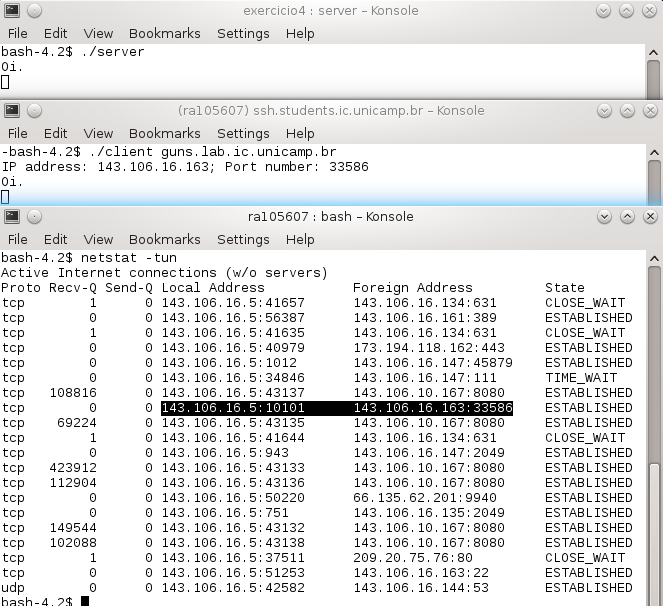
\includegraphics[width=117mm]{images/print-ipport-client.png}
  \label{print-ipport-client}
\end{figure}



\FloatBarrier
\section{}
\paragraph{}A figura \ref{print-ipport-server} mostra tanto o cliente como o servidor imprimindo na saída padrão o endereço IP e a porta associados ao cliente pelo sistema operacional local. O servidor está sendo executado no \emph{host} \verb|guns.lab.ic.unicamp.br| (\verb|143.106.16.5), mas agora na porta 10102, e o cliente, no \emph{host} em \verb|143.106.16.163|. O endereço IP e a porta impressas por ambos programas são confirmadas pela linha destacada na saída do comando \verb|netstat -tun|.
\begin{figure}[!ht]
  \caption{Cliente imprimindo o endereço IP e a porta.}
  \centering
  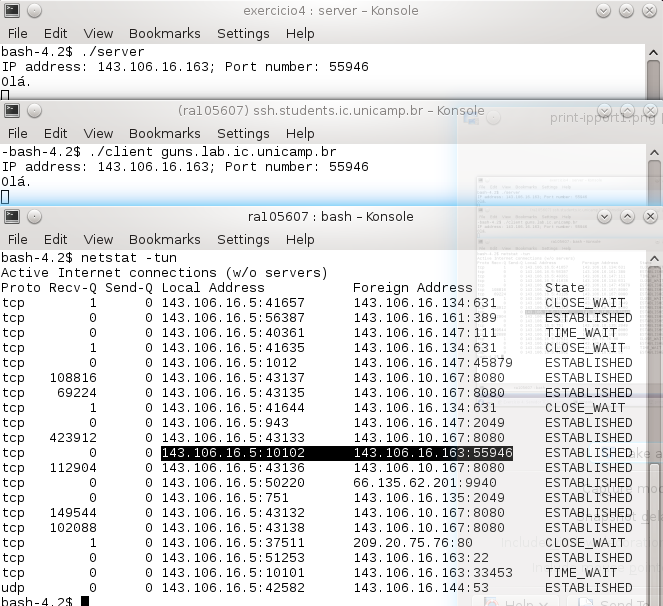
\includegraphics[width=117mm]{images/print-ipport-server.png}
  \label{print-ipport-server}
\end{figure}



\FloatBarrier
\section{}
